\documentclass[crop]{standalone}
\usepackage{tikz}
\usepackage{pgfplots}
\pgfplotsset{compat=1.15}
\usepackage[]{amsmath}
\usepackage[]{libertine}
\usepackage[libertine]{newtxmath}
\usepackage[]{bm}
\usepackage[]{physics}
% Typographical refinement
\usepackage[activate={true,nocompatibility},% Let microtype do its magic
%                                           % without trying to keep page breaks
%                                           % etc.
final=true,% Activate microtype even when in draft mode
kerning=true,% Fixes kerning issues
spacing=true,% Fixes spacing issues
tracking=true,% Adds letter spacing for small caps
shrink=30,% Characters are stretched or shrunk in order to improve justification
stretch=30,% up to 3 %
factor=0% Controls how much punctuation protrudes past the end of the line
]{microtype}
\microtypecontext{spacing=nonfrench} % <-- No spacing found for Linux Libertine
% Macros for greek letters in roman style, in math mode
\DeclareRobustCommand{\mathup}[1]{%
\begingroup\ensuremath\changegreek\mathrm{#1}\endgroup}
\DeclareRobustCommand{\mathbfup}[1]{%
\begingroup\ensuremath\changegreek\bm{\mathrm{#1}}\endgroup}


\makeatletter
\def\changegreek{\@for\next:={%
        alpha,beta,gamma,delta,epsilon,zeta,eta,theta,iota,kappa,lambda,mu,nu,%
        xi,pi,rho,sigma,tau,upsilon,phi,chi,psi,omega,varepsilon,varpi,%
    varrho,varsigma,varphi}%
\do{\expandafter\let\csname\next\expandafter\endcsname\csname\next up\endcsname}}
\makeatother

% Define vectors in bold, roman, lowercase font
\newcommand{\vct}[1]{\ensuremath{\mathbfup{\MakeLowercase{#1}}}}

% Define unit vectors in bold, roman, lowercase font, with hats
\newcommand{\uvct}[1]{\ensuremath{\mathbfup{\hat{\MakeLowercase{#1}}}}}

% Define matrices in bold, roman, uppercase font
\newcommand{\mtrx}[1]{\ensuremath{\mathbfup{\MakeUppercase{#1}}}}
\usetikzlibrary{%
    shapes,%
    arrows,%
    positioning,%
    calc%
}

\tikzset{
    block/.style = {draw, rectangle, stroke = black!80,fill = gray!15, minimum
    height = 3em, minimum width = 6em},
    arr/.style = {single arrow, draw, ->}
}
\begin{document}
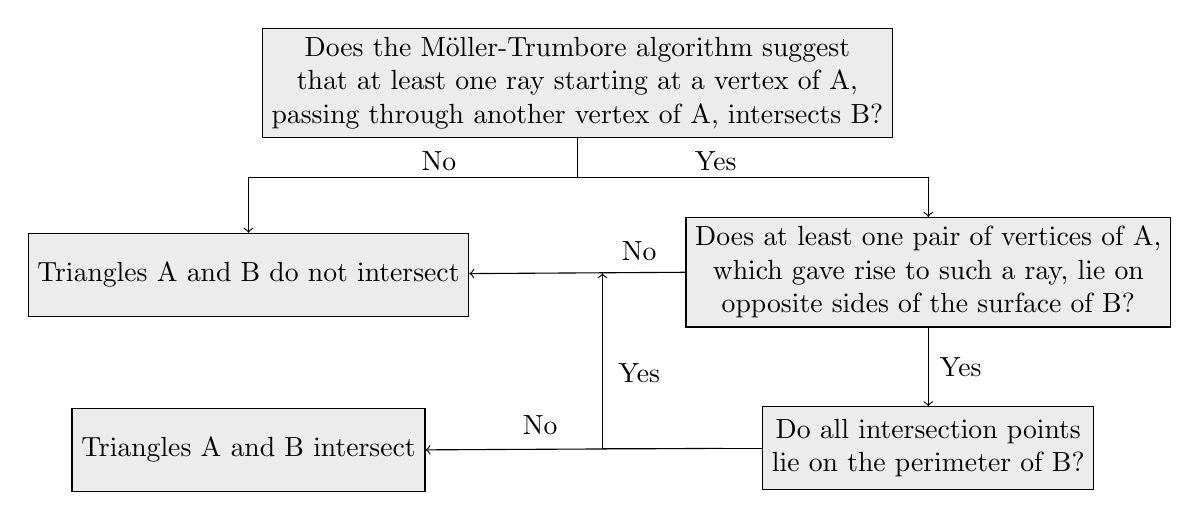
\begin{tikzpicture}
    \node[align=center] (initial) [block] {Does the M{\"o}ller-Trumbore algorithm suggest \\that at least one ray starting at a vertex of A,\\passing through another vertex of A, intersects B?};
    \node[align=center,below right= and -75pt of initial] (deeper) [block] {Does at least one pair of vertices of A,\\which gave rise to such a ray, lie on\\opposite sides of the surface of B?};
    \node[align=center,below left= 34.2pt and -75pt of initial] (nope) [block] {Triangles A and B do not intersect};
    \node[align=center,below = 32.8pt of nope] (yep) [block] {Triangles A and B intersect};
    \node[align=center,below = of deeper] (deepest) [block] {Do all intersection points\\ lie on the perimeter of B?};
    \draw[arr] (initial.south) -- ++(0,-0.5) node [auto, swap, xshift = 50, yshift = 6] {Yes} -| (deeper.north);
    \draw[arr] (initial.south) -- ++(0,-0.5) node [auto, swap, xshift = -50, yshift = 6] {No} -| (nope.north);
    \draw[arr] (deeper.south) -- node [auto, swap, xshift = 30, yshift = 0] {Yes} (deepest.north);
    \path[->] (deeper.west) edge (nope) node [auto, swap, xshift=-30, yshift=7.5] (q) {};
    \node[align=center, right = 0pt of q] (k) {No};
    \node[align=center, below = 30pt of k] (l)  {Yes};
    \node[align=center, below left = 5pt and 15pt of l]  {No};
    \draw[arr] (deepest.west) -- ++(-0.5,0) -| ($(q)+(0,-0.275)$);
    \path[->]  (deepest.west) -- ++(-0.5,0) edge (yep.east);


\end{tikzpicture}
\end{document}
